\section{eXtended Markup Language}
This chapter concerns some information our group has collected during the XML labs. The week assignments are described in the first subsection, while section \ref{subsection:soap} describes the SOAP protocol.

\subsection{Assignments}
Below are all the XMl assignments of week 1.

\subsubsection{Assignment 1}
 A federated wiki enables users to fork existing pages and modify it to their own extent. Unlike a traditional wiki, the original page won't be modified when saving the user's content. Instead, a new, `forked` page has been created alongside the original page. The new page is just as easy to find as the original page, and is still hosted on the same wiki platform. This solves a problem where multiple editors of the same page conflicted on the contents to display on certain pages.

\subsubsection{Assignment 2}
The XML and DTD for this assignment were validated on Validome.org , as to be seen in figure \ref{fig:xmldtdtest}. The XML code for this assignment can be found in attachment \ref{appendice:xmldtdsrc}.
\begin{figure}[H]
	\centering
	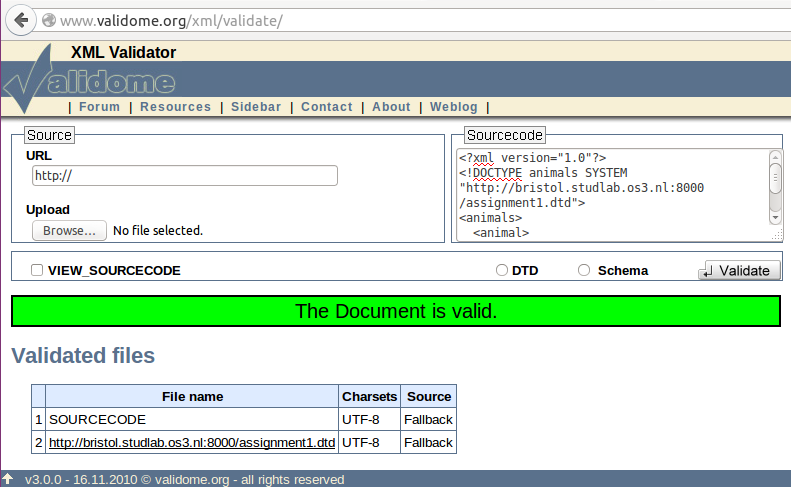
\includegraphics[width=100mm]{img/xmldtdtest.png}
	\caption{Test results of the DTD file}\label{fig:xmldtdtest}
\end{figure}

For the XML schema, I used the schema validator from utilities-online. The proof is to be seen in figure \ref{fig:xmlxsdtest}.

\begin{figure}[H]
	\centering
	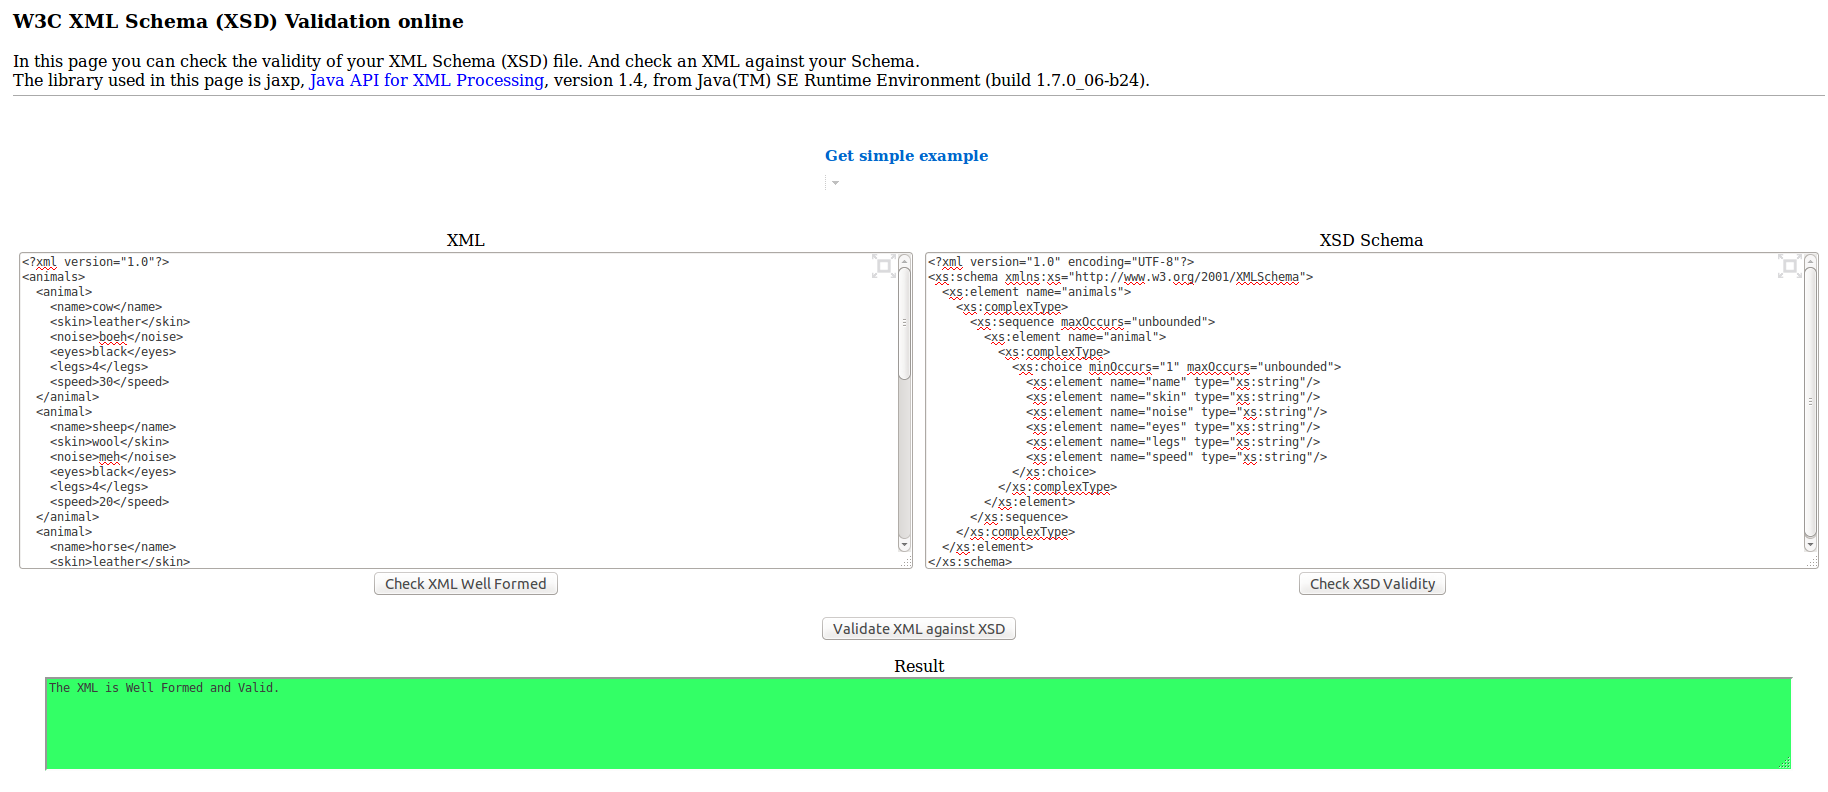
\includegraphics[width=100mm]{img/xmlxsdtest.png}
	\caption{Test results of the XML XSD schema}\label{fig:xmlxsdtest}
\end{figure}

\subsubsection{Assignment 3}
I validated this assignment on w3schools. For the result, check figure \ref{fig:xhtml}.

\begin{figure}[H]
	\centering
	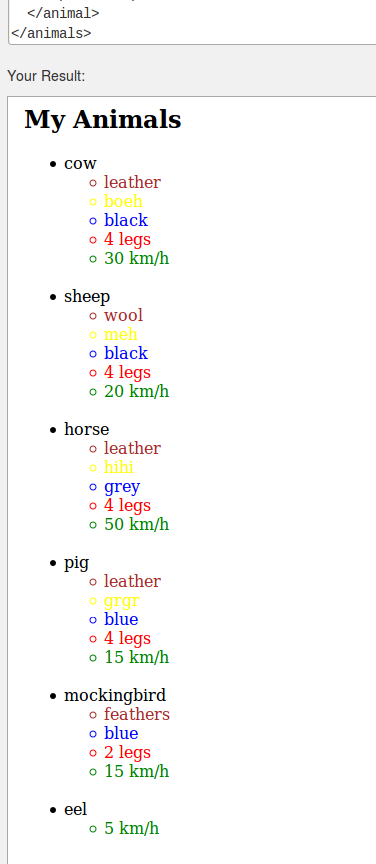
\includegraphics[height=80mm]{img/xhtml.png}
	\caption{Test results of my XHTML and CSS}\label{fig:xhtml}
\end{figure}

\begin{minted}{xml}
<?xml version="1.0" encoding="UTF-8"?>
<xsl:stylesheet version="1.0" xmlns:xsl="http://www.w3.org/1999/XSL/Transform">

<xsl:template match="/">
  <html>
  <head>
  <style type="text/css">
    li.name {
      color: black
    }
    li.noise {
      color: yellow
    }
    li.skin {
      color: brown
    }
    li.eyes {
      color: blue
    }
    li.legs {
      color: red
    }
    li.speed {
      color: green
    }
    li:hover {
      color: grey
    }
  </style>
  </head>
  <body>
  <h2>My Animals</h2>
      <ul>
        <xsl:for-each select="animals/animal">
        <li class="name"><xsl:value-of select="name"/></li>
        <ul>
          <xsl:if test="skin"><li class="skin"><xsl:value-of select="skin"/></li></xsl:if>
          <xsl:if test="noise"><li class="noise"><xsl:value-of select="noise"/></li></xsl:if>
          <xsl:if test="eyes"><li class="eyes"><xsl:value-of select="eyes"/></li></xsl:if>
          <xsl:if test="legs"><li class="legs"><xsl:value-of select="legs"/> legs</li></xsl:if>
          <xsl:if test="speed"><li class="speed"><xsl:value-of select="speed"/> km/h</li></xsl:if>
        </ul>
        <br/>
        </xsl:for-each>
      </ul>
  </body>
  </html>
</xsl:template>
</xsl:stylesheet>
\end{minted}

\subsection{Simple Object Access Protocol}\label{subsection:soap}
SOAP stands for Simple Object Access Protocol, and offers a way for applications to interact with one another. It extensively uses XML to wrap up it's messages. The SOAP standard defines a couple of characteristics. First, every SOAP call is wrapped in an Envelope. Inside the Envelope, a Header may or may not be present. The Header may contain additional information belonging to the request, for example authentication information or preferences. The second element in the Envelope is the Message. This element contains the actual request from the client, or response from the server.

As I wanted to see how a simple SOAP interaction would look like, I created two Python scripts. One sets up an HTTP server and serves a SOAP accessible function. The seconds scripts initiates a client request. The function published by the SOAP server is calculating the square root of a given value.

As to be seen in the code blocks below, the client asks the server to calculate the square root of 9. The server has wrapped it's response to the request in a calculateRootResponse XML element, which contains one sub element. Namely, the outcome of the calculateRoot function. The nice thing to see here, is that the response of the server is treated like a regular Python object. The response.squareRoot contains the response of the server. The scripts were created with the help of the pysimplesoap package.

I found SOAP very easy to use myself. However, the overhead for using SOAP is quite large. According to Wikipedia, financial institutions experienced their message size increased by four times after switching from CDR to SOAP. This can be an argument against using SOAP when trafficking large amounts of data.

\subsection{Experimenting}
As we would like to see how SOAP works, we set up a client-server testapplication in Python. Below is the code for the server.

\begin{minted}{python}
#!/usr/local/bin/python
 
from pysimplesoap.server import SoapDispatcher, SOAPHandler
from BaseHTTPServer import HTTPServer
from math import sqrt
 
def calculateRoot(value):
  return sqrt(value)
 
dispatcher = SoapDispatcher(
    'root_dispatcher',
    location = 'http://localhost:8000/',
    action = 'http://localhost:8000/',
    namespace = 'http://bristol.studlab.os3.nl/root.wsdl', prefix='ns0',
    trace = True,
    ns = True)
 
dispatcher.register_function('calculateRoot', calculateRoot,
    returns = {'squareRoot': float},
    args = { 'value': float })
 
print 'Starting HTTP server'
server = HTTPServer(("", 8000), SOAPHandler)
server.dispatcher = dispatcher
server.serve_forever()
\end{minted}

\paragraph{Client Application}\mbox{}\\
Below is our client application. Pimped with the minted package for \LaTeX.

\begin{minted}{python}
#!/usr/local/bin/python
 
from pysimplesoap.client import SoapClient, SoapFault
 
client = SoapClient(
  location = "http://localhost:8000/",
  action = 'http://localhost:8000/',
  namespace = "http://bristol.studlab.os3.nl/root.wsdl", 
  soap_ns='soap',
  trace = True,
  ns = False)
 
response = client.calculateRoot(value=9)
 
result = response.squareRoot
print float(result)
\end{minted}
